\chapter{Approach}

\section{Solution Strategy} 

This project’s goal is to distinguish contrails from the clouds, so we started by thinking about the main difference between the graphs of contrails and clouds. \\
Contrails usually show as a line on the image. Meanwhile, the clouds layout in a random discrete distribution. In this way, we can write a program to detect the straight lines in images to recognize the contrails. \\
However, it should be realized that even when the contrails look like pencil lines on the image, there doesn’t exist an actual straight line when scanning through the image data. Contrails also have some width in the image (in the real world, contrails could be several kilometers in width (CONTRAILS FACTS, page 3)). The real shape of contrails seems more like some long and thin rectangles with two fading sides. In this case, the detection problem became much harder. \\
Since this solution is hard to compute, instead of detecting the contrails’ width, it is much easier to just detect the two clear sides of contrails. In this case, we can ignore the image inside the contrails, as well as other pixels inside the cloud by doing the edge detection.\\
After performing the edge detection, we can detect lines by Hough Transform on the edgel map. Another problem was that there were too many edge pixels in the image (see the result by … below). Those bad edgels came to the Hough Transform to give incorrect lines, which do not come from contrails.\\
To solve this problem, some processing on the edge image to get rid of bad edge pixels is necessary. In order to delete those bad edge pixels from clouds or other graphics, each pixel with a certain size of pixels around is checked as a small block. As lines can be divided into infinity small lines, if a line goes through a small block, there must exist a small line inside the small block. We can use polynomial curve fitting to get the slope of the best small line in each block. Then we check how well the block edgels fit the computed line. Poor fits not as determined by a line residue causes the create edgel on the block to be rejected from the further Hough Transform.\\
After this processing, use the Hough Transform, a much better result will be got.\\

Here is the whole solution:

\begin{enumerate}
    \item Convert the color image to gray-scale;
    \item Use the Canny edge detection to get the edge;
    \item Get the small blocks pixel by pixel, and do the polynomial curve fitting to get the small line information;
    \item Put all the edgels surviving the polynomial curve fitting procedure into a new image;
    \item Do the Hough Transform on new image;
    \item Median filter the new image;
    \item Plot the results.
\end{enumerate}

\section{MatLab Methods}


\subsection{Canny Edge Detection}
\vspace{3mm}
\textit{Edge\_image = edge (I, \lq{canny}\rq);}\\
\newline
\textbf{Input: I, grayscale Image}\\
\textbf{Output: Edge\_image, the black and white edge image}\\
\newline
Canny edge detection is a technique to extract useful structural information from different vision objects and dramatically reduce the amount of data to be processed. There are following steps:
\begin{enumerate}
\item Apply the Gaussian filter to remove the noise;
\item Find the intensity gradient of the image;
\item Apply non-maximum suppression to get rid of spurious response to edge detection;
\item Apply double threshold to determine potential edges to filter out the edge pixel with the weak gradient value and preserve the edge with the high gradient value;
\item Track edge by hysteresis: Finalize the detection of edges by suppressing all the other edges that are weak and not connected to strong edges.
\end{enumerate}


\subsection{Polynomial curve fitting}
\vspace{3mm}
\textit{p = polyfit(x,y,n);}\\
\newline
\textbf{Input: \\x and y, vectors containing the x and y data to be fitted;\\ n, the degree of the polynomial to return;}\\ 
\textbf{Output: p, the third-degree polynomial that approximately fits the data.}\\
\newline
This algorithm returns the coefficients for a polynomial p(x) of degree n that is the best fit (in a least-squares sense) for the data in y. The coefficients in p are in descending powers, and the length of p is n+1.


\subsection{Hough Transform and Hough Line Transform}
\begin{wrapfigure}{r}{5.5cm}
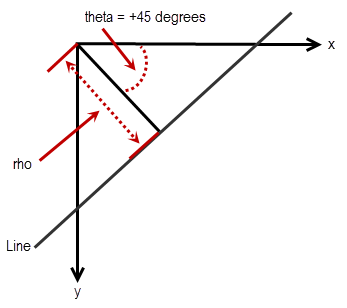
\includegraphics[width=5cm]{pic/SHT-example.png}\\
\caption{theta($\theta$) and rho($\rho$) of Hough Transform}
\end{wrapfigure}
\vspace{3mm}
\textit{[H,theta,rho] = hough(BW);}\\
\newline
\textbf{Input: BW, the black and white image;}\\
\textbf{Output:\\ H, the Hough Transform matrix be returned as a numeric array;}\\ 
\textbf{theta($\theta$), the angle in degree between the x-axis and rho vector;}\\
\textbf{rho($\rho$), the distance from origin to the line along a vector perpendicular to the line;}\\
\newline
The Standard Hough Transform (SHT) uses the parametric representation of a line: \begin{center} $\rho$ = xcos$\theta$ + ysin$\theta$.\end{center} 
For each pixel of the image, numbers of lines going through it with all different angles. If they are in the same line, they will have the same rho and theta number. During the graph or different angle and distance, we will get a cross point, which means the straight line’s rho and theta.\\ 
\begin{figure}[ht]
    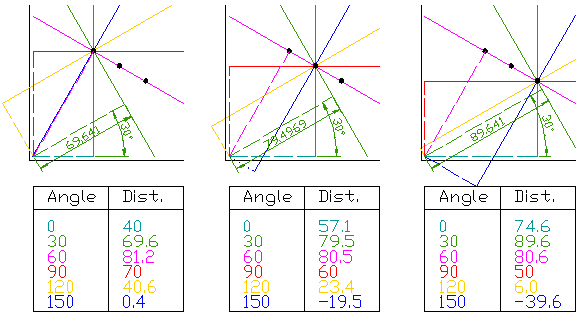
\includegraphics[scale=0.7]{pic/SHT-example2.png}
    \caption{$\theta$=60, $\rho$ are same for the 3 points}
\end{figure}
As we can see from above figure (Wikipedia.com), when the Hough Transform algorithm goes through all different angles ($\theta$) in every pixels, there is a certain angle ($\theta$ = 60 in above figure), it makes the perpendicular distance from the line to origin keeps the same ($\rho$ = 81.2 ~= 80.5 ~= 80.6). When we draw all the information below, we can have a much clear view for how the Hough Transform works.\\

\subsection{Median Filter}
\vspace{3mm}
\textit{B = medfilt2(A, [m n]);}\\
\newline
\textbf{Input:\\ A, the original image;}\\
\textbf{[m n], the isolate pixels’ size to be deleted;}\\ 
\textbf{Output: B, the image after deleted the isolated pixels.}\\
\newline
Put m x n pixel values around each target pixel into an array, then order all the values in the array, after this, we find the median value of the array and put it into the target pixels.

\section{Algorithm to reduce the bad edgels}

\subsection{Describe}
\textbf{This is a script, the input will be the edge image, and the output will delete the little block contains the small enough residual values.}\\
Since the Canny edge detection gives many edgels we need to further process these edge maps to eliminate edgels (edge pixels) that are not parts of straight lines. For each $2\times s$+1 by $2\times s$+1 square neighborhood about a pixel, we fit all the neighborhood edgels to a straight line using polyfit. We fit either y=mx+b for lines where $\left|m\right|$ $\leq$ 45 degrees and x=$\frac{y-b}{m}$ if $\left|m\right|$ $\geq$ 45 degrees. This takes care of horizontal and vertical lines. Now we have the equation of the best line fit for all the edgels in a neighborhood. But how good is this line fit? For each neighborhood edgel we compute the residual of that edgel’s neighborhood fit to the line. We compute the overall residual as the square root of the sum of these squared residual values.\\
Since neighborhoods with poor line fits will have large overall residual values, we remove bad edgels using a threshold of 15 determined by trial and error.

\subsection{Pseudo code}
\begin{lstlisting}[language=Java]
I = Read image;
grayscale (I);
image = Canny edge detect(I);
set the block size, height and width (s, height, width)
	
initial number no lines = 0;

for x = (1+s) to (height-s):
    for y = (1+s) to (width-s):
    initial points number = 0:
        if pixel is on an edge:
            for i = (x-s) to (x+s):
                for j = (y-s) to (y+s):
        	        if block pixel is edge:
                        record them;
                        points number ++;
        	if at least one line in a block:
        	    m = polyfit (x and y data recoded);
        	    if (line’s slope >1 or <-1):
        	        compute the residual r;
        	    else:
        	        modify the m;
        	        compute the residual r;
        	    save r values
        	else:
                number no lines ++;
                
get non_zero_r;
sort non_zero_r;	
set the precentage p;
threshold = cast(p% * non_zero_r);


for x = (1+s) to (height-s):
    for y = (1+s) to (width-s):
        if the r value is in the shreshold and non zero:
	        write it on new_image;
	        
new_image = medfilter (new_image);
get Hough Transform matrix(H), theta(T) and rho(R) by hough(new_image);
get peaks(P) = houghpeaks (new_image);
lines = houghlines(new_image, T, R, P);

for k = 1 to number of lines:
    plot lines on origin image(I);

\end{lstlisting}